\section{Ordering and Asynchrony}
\label{sec:async}

\begin{figure}[t]
  \centering
  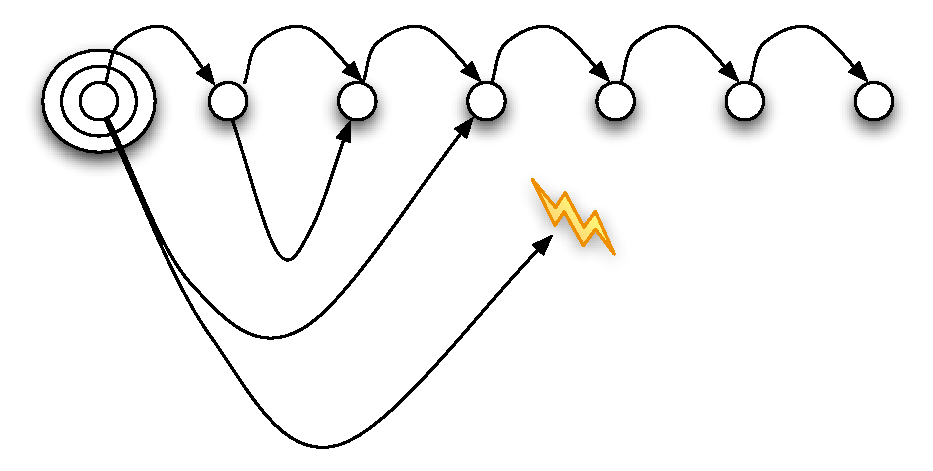
\includegraphics[width=0.75\linewidth]{figures/dedalus-time.pdf}
  \label{fig:time}
  %%\caption{Time moves forward in three ways: across strata, to the next fixpoint, and to some future fixpoint.}
   \caption{Dedalus admits inferences whose consequences are visible immediately, in the next timestep, or at some unspecified timestep.}
   
\vspace{-8pt}
\end{figure}

Until now we have restricted our discussion to \slang.  In this section we
consider \lang, a superset of \slang that admits aggregate functions
and the \emph{choice} construct.  These constructs will allow us to
express programs that establish or enforce an ordering over inputs, and to
reason about the inherent nondeterminism in communication over unreliable
networks that may delay, lose or reorder the results of logical deductions 
(see Figure~\ref{fig:time}).

\subsection{New Constructs}

In this section we relax our restrictions on \slang by admitting aggregate functions to 
capture ordering constraints, and the choice construct to capture nondeterminacy.

\subsubsection{Aggregate Functions}

We will consider only the class of \emph{exemplary} aggregate
functions~\cite{tag} -- an exemplary aggregate function's codomain is a subset
of its domain. 
%%-- and the \emph{count} aggregate, which is expressible using arithmetic.  
We allow exemplary or count aggregate functions $\rho_1 - \rho_n$ to appear
in the head of a deductive rule of the form:

\dedalus{p(\(A_1\), \(\ldots\), \(A_n\), \(\rho_1\)(\(A_{n+1}\)), \(\ldots\), \(\rho_m\)(\(A_{n+m}\))) \(\leftarrow\)}
\linebreak\dedalus{   \(q_1\)(\(A_1\), \(\ldots\), \(A_n\)), \(\ldots\), \(q_n\)(\(A_1\), \(\ldots\), \(A_n\));}

These functions do not affect the expressivity of the language; we admit them
to simplify our discussion of ordering.  It is easy to see that the \emph{min} function,
which we subsequently use, is expressible in Datalog using negation.

%%\begin{example}
%%The query below selects, for each distinct value of the first column of $p$, the minimum 
%%value of the second column.

%%\begin{Dedalus}
%%min_p(A, min<B>) \(\leftarrow\) p(A, B);
%%\end{Dedalus}

%%The Datalog program below is equivalent:

%%\begin{Dedalus}
%%notmin_p(A, B) \(\leftarrow\) p(A, B), p(A, C), B > C;
  
%%min_p(A, B) \(\leftarrow\) p(A, B), \(\lnot\)notmin_p(A, B);
%%\end{Dedalus}
%%\end{example}




%%\dedalus{r\pos($A_1$, $A_2$, [...], $A_n$, }

%%$\rho$($A_{n+1}$)}

%%$\rho$($A_{n+2}$), [...] $\rho$($A_{n+m}$)) \(\leftarrow\) r($A_1$, $A_2$, [...], $A_n$);}



\subsubsection{Choice}

We also admit the \emph{choice} construct as defined by Greco and Zaniolo~\cite{greedychoice}.
The subgoal \dedalus{choose((\emph{$X_1$}), (\emph($X_2$))} may appear in the body of a rule, where
\emph{$X_1$} and \emph{$X_2$} are vectors of variables occuring also elsewhere in the body.  Such a subgoal
enforces the functional dependency \emph{$X_1$} $\to$ $X_2$, ``choosing" a single assignment of values to the variables
in \emph{$X_2$} for each variable in \emph{$X_1$}.

The choice construct is nondeterministic.  In a model-theoretic interpretation of logic programs, a nondeterministic program 
must be one that has a multiplicity of stable models -- that is to say, an unstratifiable program.  Greco and Zaniolo define 
choice in precisely this fashion: the choice construct is expanded into an unstratifiable rule clique, 
and each possible choice is associated with a different model.

\paa{significantly, for any choice, the resulting program has a unique minimal model if the program (independent of the choice expansion)
is stratifiable, locally stratifiable, etc}


\subsection{Distribution Model}

A principal motivation for the specification of \lang is modeling and implementing distributed systems.
To represent such a system we must consider a multiplicity of asynchronous agents evaluating local programs and
communicating via messages.  As with previous distributed logic languages, we model messages as
tuples and their transmission as a special case of rule evaluation in which the body is evaluated at one
agent and the head atom appears at another.  

An agent clearly cannot evaluate rules whose body
predicates exist at another agent, and hence these message rules are the only manner in which data
elements derived from one agent's EDB may be visible in the IDB of another.  This restriction is 
particularly significant to our interpretation of timestamps.  Although the \emph{successor} relation exists
at each agent according to our definition, there is no reason to assume that a subset of that relation 
relevant to computation at any particular agent will intersect the relevant subset at another.  In other words,
if we consider the ``current local time" as a pointer to a particular row of successor, we must admit that in a 
distributed system, each agent's pointer will likely point to a different row, and there is certainly no way for
a given agent to know the value pointed to by another.

It follows that a message rule as described above will deduce a head predicate whose timestamp is independent
of the timestamps in the body predicates, and which cannot have been predicted by the agent at which the rule
was evaluated.

\subsection{Asynchronous Rules}

%%\rcs{ I touched this.  There is no longer a time predicate, we no longer admit causality violations}

In order to represent the nondeterminism introduced by distribution, we admit a
third type of rule, called an {\em asynchronous} rule.  A rule is asynchronous
if the 
%Recall our use of the distinguished variables $\Tau$ and $S$ to represent the
%time suffixes respectively in the body and head of a rule
%(Section~\ref{sec:syntaxrestrictions}).  in our discussion of \slang,
%representing the time suffixes occuring respectively in the body and head of a
%rule.
relation between the head time suffix $S$ and the body time suffix $\Tau$ is
unknown.  Furthermore, $S$, but not $\Tau$, may take on the special value
$\perp$ which means ``never.''  Derivation at $\perp$ indicates that the
deduction is ``lost,'' as time suffixes in rule bodies do not range over
$\perp$.

We model network nondeterminism using the \dedalus{choice} construct to choose
from a value in the special 
%%\dedalus{successors} 
\dedalus{time}
predicate, which is defined using the following datalog rules:

\begin{Dedalus}
time(\(\perp\));
time(S) \(\leftarrow\) successor(S, _);
\end{Dedalus}


Each asynchronous rule has the following additional variables in its
body: \dedalus{time(S), choose((\_), (S))}, where
$\SDedalus$ is the timestamp of the rule head.

\begin{example}
A well-formed asynchronous \lang rule:

\begin{Dedalus}
r(A, B, S) \(\leftarrow\) 
  e(A, B, \(\Tau\)),
  time(S), choose((_)), (S));
\end{Dedalus}
\end{example}

We admit a new temporal head annotation to sugar the rule above.  The
identifier \dedalus{async} implies the rule is asynchronous, and stands in for the additional body predicates.
%%$N$ is a variable,
%%corresponding to the time suffix $\Tau$ of all predicates in the rule body and
%%optionally referenced in the head.  
The above example expressed using \dedalus{async} is:

\begin{Dedalus}
asynchronous
r(A, B)@async \(\leftarrow\) e(A, B);
\end{Dedalus}

It is easy to see that evaluation of an asynchronous rule may produce a tuple whose timestamp is less than $\Tau$, the timestamp
in the rule's antecedents. 
%%This violates our intuitive interpretation of timestamps capturing causal relations between 
%%tuples, and compromises the temporal stratifiability proof of \slang, because it is no longer the case that a ground atom
%%cannot possibly depend negatively on itself.
This violates the monotonicity assumptions upon which we based our proof of temporal stratification, and muddies our interpretation
of timestamps as capturing causal relations between tuples.


\subsubsection{Later: Causally-Constrained Asynchrony}

Ultimately, whether a particular set of temporal semantics is
desirable depends on the underlying application; for example, clever
combinations of crash-prone databases running ``read uncommitted''
transactions and asynchronous event queues can easily suffer from
grandfather paradoxes and other temporal impossibilities.  

%%\rcs{move this, get rid of monotonic discussion?
%%We observe, however, that the order of evaluation of a Datalog program is irrelevant to the final result when the program is 
%%purely monotonic.  For such a program~\footnote{This holds also for the trivial cases of programs that ignore messages.}, 
%%deductions ``into the past" present no difficulties.
%%In fact, the ``eventual consistency" property of NDLog~\cite{loo-sigmod06} relies on the assumption that
%%programs are negation-free and hence monotonic.  Any programs with non-monotonic rules that transitively depend on
%%message tuples, however, may need to enforce an ordering discipline on such tuples.  We discuss this in detail in Section (Lamport Clocks).
%%}

The distributed systems literature typically assumes a causal ordering
of events across systems; Lamport clocks are a simple mechanism that
records the partial ordering induced by network communication between
the nodes.  With such approaches in mind, we introduce an alternative
to \dedalus{@async} called \dedalus{@later} that induces a total
ordering over all timestamps within a \lang program.  Instead of \dedalus{time}, we define \dedalus{after}:

\begin{Dedalus}
after(S, T) \(\leftarrow\) successor(S, T);
after(S, U) \(\leftarrow\) after(S, T), successor(T, U);
after(S, \(\perp\)) \(\leftarrow\) successor(S, _);
\end{Dedalus}

Intuitively, \dedalus{after(S, T)} is true if T happens after S in the
global ordering of events.  Each \dedalus{@later} rule has the
following additional variables in its body:
\dedalus{after($\Tau$, S), choose(($\Tau$), (S))}, where, as
above, $\Tau$ is the timestamp associated with the rule body, and
\dedalus{S} is the timestamp of the rule head.

Note that our addition of a global ordering does not expose a shared
synchronized clock to \lang programs.  The nondeterminism associated
with choice prevents programs from ensuring that operations are
performed in lock-step.  Instead, the timestamps simply encode some
logical clock that is equivalent to one that could be maintained by
the application.  The difference is that, by constraining
\dedalus{choose}, we can avoid reasoning about program traces that
contain paradoxes such as causality loops.  In particular, deterministic programs such as:

\begin{Dedalus}
r(1)@1;
s(1);
p(X) \(\leftarrow\) q(X), r(X);
q(X)@later \(\leftarrow\) s(X);
\end{Dedalus}
are non-deterministic if \dedalus{@later} is replaced with
\dedalus{@async}.  
\paa{the rest may stay but may also go}
The non-determinism comes from \dedalus{@sync}'s
\dedalus{choose} invocation.  However, the non-determinism also relies
on the fact that the program is, in some sense, non-monotonic; it
relies on the fact that \dedalus{r(1)} stops being true before
\dedalus{q(1)} is derived.

%%\rcs{Can we prove anything now?  It seems as though async rules are equivalent to \slang rules, as long as there is no aggregation or arithmetic.  The problem is that if %%choice derives a fact N steps in the future, we need to push the fact through N @next rules, and the number of such rules is variable.  If we admit arithmetic in the rewrite, %%%we can model async as a synchronous queue, but \slang doesn't have arithmetic...}
%%\rcs{Here to end of section is dead text}





%\dedalus{time(t)} is true if $t \in \mathbb{Z} \cup \perp$. 
%%\rcs{didn't understand the $\Theta$ thing; kill this paragraph?}
%%An asynchronous rule has the following
%%subgoals in its body: \dedalus{time(S), successors($\Theta$, S), choose(($\Theta$), (S))}, where
%%$\Theta$ is a vector containing all variables appearing in the rule body,
%%including $\Tau$.  The choice subgoal expresses that the rule head may be
%%derived at any value of \dedalus{time}.
%time value that appears in the \dedalus{successor} relation.

%%\rcs{old example:}

%%\begin{Dedalus}
%%asynchronous
%%r(A, B, S) \(\leftarrow\)
%%   e(A, B, \(\Tau\)), successor(_, S), choose((A, B), (S));
%%\end{Dedalus}


\subsubsection{Entanglement}

Consider the asynchronous rule below:

\begin{Dedalus}
p(A, B, N)@async \(\leftarrow\)
  q(A, B)@N;
\end{Dedalus}

Due to the async keywork in the rule head, the \emph{p} tuple will take some unspecified time suffix value.
Note however that the time suffix $N$ of the rule body appears also in the \emph{p} tuple, capturing a 
binding between the time value of the deduction and the time value of its consequence.  We call such a binding
an \emph{entanglement}.   Entanglement is a surprisingly powerful construct that allows a rule to 
reference the logical clock time of the deduction that produced one (or more) of its subgoals.  Note that in order
to write the rule it was necessary to not sugar away the time suffix in the rule body.  Entanglements are only 
permitted in asynchronous rules.

\subsection{Distributed Programs}

A distributed \lang program consists of a set of predicates \emph{P} partitioned across a set of hosts \emph{H}.
%%Consider two hosts $a$ and $b$ in \emph{H}, and two predicates $p$ and $q$ in \emph{P}.  Without loss of generality, 
%%we call an async rule $r$ a \emph{communication rule} if $p$ is defined at $a$ and $q$ is defined at $b$, $p$ occurs in the  
A \emph{communication rule} is an asynchronous rule whose head predicate is defined at a different host than its body predicates,
all of which are defined at a single host.  

It is easy to see that the only mechanism for sharing data between agents in a distributed system is through such communication 
rules.  Because communication rules (being asynchronous) cannot themselves capture causality relationships between tuples
via timestamps, any necessary relationship must be encoded into the tuples themselves via an entanglement.


\subsection{Ordering and distribution in Logic}

\subsubsection{Sequences}

One may represent a database sequence -- an object that retains and monotonically increases a counter value -- 
with a pair of inductive rules.  One rule increments the current counter value when some condition is 
true, while the other persists the value of the sequence when the condition is false.  We can capture the increase
of the sequence value without using arithmetic, because the infinite series of \emph{successor} has the monotonicity
property we require.  We need only to entangle the time suffix into the tuple:

\begin{Dedalus}
seq(A, N)@next \(\leftarrow\) seq(A, _)@N, event(A)@N;
  
seq(A, X)@next \(\leftarrow\) seq(A, X), \(\lnot\) event(A);
\end{Dedalus}

%%We must admit arithmetic functions into our language to express such a
%%sequence, but the pair of rules above remains temporally safe.

Clearly, to implement a sequence that increases consecutively without gaps would require using arithmetic.


\subsubsection{Queues}

%%Consider a trace of events to a 
Consider a predicate \dedalus{balance\_update} that represents updating the a
user's account balance.  Its attributes are a string representing a user, a
floating point number indicating a new account balance and an integer
indicating the order in which the updates were issued, according to some
external clock or sequence:

\begin{Dedalus}
balance\_update("bob", 100.00, 2355)@123;
balance\_update("bob", 75.00, 2358)@123;
balance\_update("alice", 0.00, 2377)@123;
balance\_update("bob", 10.00, 2455)@123;
\end{Dedalus}

Note that all the time suffixes are the same.  
%Depending on the program that implements the balance update, several behaviors
%are possible.
Given this schema, we note that a program would likely want to process
\dedalus{balance\_update} events individually in a data-dependent order, in
spite of their coincidence in logical time.  It is difficult to express general
in-order tuple processing in Datalog, in part because the language does not
admit sequences.
%above is really what we want to say, right? -wrm
%has so
%notion of order of evaluation (except the implicit ordering implied by
%stratification).

In the program below, we define a table \dedalus{m\_balance\_update} that
serves as a queue to feed \dedalus{balance\_update}.  The queue must persist
across timesteps because it may take multiple timesteps to drain it.  At each
fixpoint, for each value of \textbf{A}, a single tuple is projected into
\dedalus{balance\_update} and deleted (atomic with the projection) from
\dedalus{m\_balance\_update}, changing the value of the aggregate calculated
at the subsequent step:

\begin{Dedalus}

m\_balance\_update(A, B, C)@next \(\leftarrow\)
  m\_balance\_update(A, B, C),
  notin del\_m\_balance\_update(A, B, C);

omin(A, min<C>) \(\leftarrow\)
  m\_balance_update(A, _, C);

p(A, B, C)@next \(\leftarrow\)
  m\_balance\_update(A, B, C),
  omin(A, C);

del\_m\_balance\_update(A, B, C) \(\leftarrow\)
  m\_balance\_update(A, B, C),
  omin(A, C);
\end{Dedalus}

Under such a queueing discipline, deductive rules that depend on
\emph{balance\_update} are constrained to consider only one tuple per fixpoint
per value of the variable \textbf{A}, thus implementing a per-user FIFO
discipline.  To enforce a global FIFO ordering over \emph{balance\_update}, we
may redefine \emph{omin} and any dependent rules to exclude the \textbf{A}
atttribute.

A queue establishes a mapping between the local clock and the ordering domain of the input relation. By doing so, we are able to take
advantage of the natural ordering enforced by stratification over time, to enforce an ordering property over our input that is otherwise 
very difficult to express in a logic language.

\subsubsection{Lamport Clocks}

Implementing a Lamport Clock~\cite{timeclocks} is a special case of a queueing discipline as defined above.
Consider a predicate{m\_balance\_update} as defined above, but with an extra integer attribute that contains the logical transmission
time of the sender (via a message rule) of a given tuple.  For example, the sender's rule will look like: 

\paa{damn it!  we've sugared out N from the syntax!! now what?}
\rcs{perhaps this would be better without the balance update example... I think they'll get that lamport clocks are useful}

Consider a rule:
\begin{Dedalus}
x(A, B) :- y(A, B);
\end{Dedalus}
whose productions should be annotated using a Lamport clock.  We add a
third column to x and y that will track the logical timestamps of the
productions.  With entanglement, we would simply write:

\begin{Dedalus}
entangle
x(A, B, N) :- y(A, B, M)@N;
\end{Dedalus}

which would store the derivation time of \dedalus{x}.  Note that no explicit
increment of \dedalus{N} is required.  If \dedalus{M} is set according to a similar
rule, then we know that \dedalus{N} $\ge$ \dedalus{M}, due to the semantics of
\dedalus{@next} and \dedalus{@async}.

Alternatively, the program could maintain the clock values manually,
with rules such as:

\begin{Dedalus}
x(A, B, M+1) :- y(A, B, M), \(\neg\)x(_, _, _);
x(A, B, max<M,N>+1) :- y(A, B, M), x(_,_,N); 
\end{Dedalus}
\rcs{max syntax is cheating, and the rewrite is horribly broken.  However, I'd like to introduce a non-entangled lamport clock in order to motivate entanglement.  FIXME or get rid of everything after ``entanglement''}

This avoids the use of entanglement, but requries aggregation and
arithmetic.  Also, if a cycle exists between x and y; the rewrite's
use of addition may be unsafe.

  \rcs{end potential
  rewrite}

\begin{Dedalus}
entangle
m\_balance\_update(A, B, N)@async \(\leftarrow\)
  send\_p(A, B)@N;
\end{Dedalus}

Note that in the rule named \emph{entangle}, the time suffix is projected into the last attribute of \emph{m\_p}.  
This establishes an \emph{entanglement} between
the sender's local clock and the program dataflow.  The queueing discipline that implements a
Lamport clock is then:

\begin{Dedalus}

m\_balance\_update(A, B, C)@next \(\leftarrow\)
  m\_balance\_update(A, B, C),
  \(\lnot\) del\_m\_balance\_update(A, B, C);

omin(A, min<C>) \(\leftarrow\)
  m\_balance\_update(A, _, C);

lmax(max<C>) \(\leftarrow\)
  m\_balance\_update(_, _, C);

disentangle
balance_update(A, B)next \(\leftarrow\)
  m\_balance\_update(A, B, C)@N,
  omin(A, C)@N,
  lmax(L)@N,
  N > L;

del\_m\_balance\_update(A, B) :-
  m\_balance\_update(A, B),
  omax(B);
  
\end{Dedalus}

Note that the rule named \emph{disentangle} references the data elements $C$ and $L$, both of which
contain timestamps, and induces a \emph{balance\_update} tuple with timestamp $N+1$ only when $N > L$,
the highest of the timestamps in its message queue.  Under the distributed systems model of Lamport clocks, 
we expect the tuples in the message queue to  be from other hosts with independent clocks, sending messages 
over a medium that can delay or reorder them arbitrarily.  In order to make the necessary comparison between local
and remote clocks, it is necessary to reference the time suffix variable directly, rather than omitting it as we have done 
in all other \lang examples.



